\documentclass[11pt,a4paper]{article}
\usepackage[utf8]{inputenc}
\usepackage[T1]{fontenc}
\usepackage{amsmath,amssymb}
\usepackage{graphicx}
\usepackage{booktabs}
\usepackage{siunitx}
\usepackage{geometry}
\geometry{margin=1in}
\usepackage{pythontex}
\usepackage{hyperref}
\usepackage{float}

\title{Color Perception\\CIE Chromaticity}
\author{Psychophysics Research Group}
\date{\today}

\begin{document}
\maketitle

\begin{abstract}
This report presents a comprehensive computational analysis of human color perception, including trichromatic cone fundamentals, CIE chromaticity systems, opponent color channels, and color vision deficiencies. We model the spectral sensitivities of L, M, and S cones, compute chromaticity coordinates in CIE 1931 color space, analyze color discrimination thresholds via MacAdam ellipses, and simulate protanopic, deuteranopic, and tritanopic color blindness. The models integrate photoreceptor physiology with perceptual color spaces to provide quantitative frameworks for understanding human color vision.
\end{abstract}

\section{Introduction}

Human color vision arises from three classes of cone photoreceptors with distinct spectral sensitivities: long-wavelength (L), medium-wavelength (M), and short-wavelength (S) cones \cite{stockman2000spectral}. The trichromatic signals are transformed into opponent color channels (red-green, blue-yellow, luminance) at the retinal ganglion and lateral geniculate nucleus stages \cite{hurvich1957opponent}. The CIE 1931 color space standardizes color specification via tristimulus values and chromaticity coordinates \cite{wyszecki2000color}. Color discrimination varies across color space, characterized by MacAdam ellipses representing just-noticeable differences \cite{macadam1942visual}. Genetic mutations causing cone photopigment deficiencies result in color vision deficiencies (CVD) affecting approximately 8\% of males and 0.5\% of females \cite{sharpe1999opsin}.

This analysis models cone fundamentals, CIE chromaticity, opponent channels, discrimination thresholds, and CVD simulations using computational psychophysics approaches.

\begin{pycode}

import numpy as np
import matplotlib.pyplot as plt
from scipy import stats, optimize, integrate
from matplotlib.patches import Ellipse
plt.rcParams['text.usetex'] = True
plt.rcParams['font.family'] = 'serif'

# Global wavelength range
wavelength = np.linspace(380, 780, 401)  # nm, 1nm resolution

\end{pycode}

\section{Cone Fundamentals}

The spectral sensitivities of human cone photoreceptors are based on Stockman \& Sharpe (2000) 2-degree cone fundamentals \cite{stockman2000spectral}:

\begin{equation}
S_i(\lambda) = \exp\left[-\frac{(\lambda - \lambda_{\text{peak},i})^2}{2\sigma_i^2}\right]
\end{equation}

where $i \in \{L, M, S\}$ denotes cone type, $\lambda_{\text{peak},i}$ is the peak wavelength, and $\sigma_i$ controls bandwidth.

\begin{pycode}
# Cone fundamentals (Stockman & Sharpe approximation)
# L-cone: peak ~565 nm
# M-cone: peak ~540 nm
# S-cone: peak ~440 nm

L_peak, M_peak, S_peak = 565, 540, 440
L_sigma, M_sigma, S_sigma = 40, 35, 20

L_cone = np.exp(-0.5 * ((wavelength - L_peak) / L_sigma)**2)
M_cone = np.exp(-0.5 * ((wavelength - M_peak) / M_sigma)**2)
S_cone = np.exp(-0.5 * ((wavelength - S_peak) / S_sigma)**2)

# Store for later use
cone_data = {
    'L': L_cone,
    'M': M_cone,
    'S': S_cone,
    'wavelength': wavelength
}

fig, ax = plt.subplots(figsize=(10, 6))
ax.plot(wavelength, L_cone, 'r-', linewidth=2.5, label='L-cone (565 nm)', alpha=0.8)
ax.plot(wavelength, M_cone, 'g-', linewidth=2.5, label='M-cone (540 nm)', alpha=0.8)
ax.plot(wavelength, S_cone, 'b-', linewidth=2.5, label='S-cone (440 nm)', alpha=0.8)
ax.set_xlabel(r'Wavelength $\lambda$ (nm)', fontsize=12)
ax.set_ylabel(r'Normalized Sensitivity $S(\lambda)$', fontsize=12)
ax.set_title('Cone Spectral Sensitivities (Stockman \\& Sharpe 2000)', fontsize=13)
ax.set_xlim(380, 780)
ax.set_ylim(0, 1.05)
ax.legend(fontsize=11, loc='upper right')
ax.grid(True, alpha=0.3, linestyle='--')
plt.tight_layout()
plt.savefig('color_perception_plot1.pdf', dpi=150, bbox_inches='tight')
plt.close()
\end{pycode}

\begin{figure}[H]
\centering
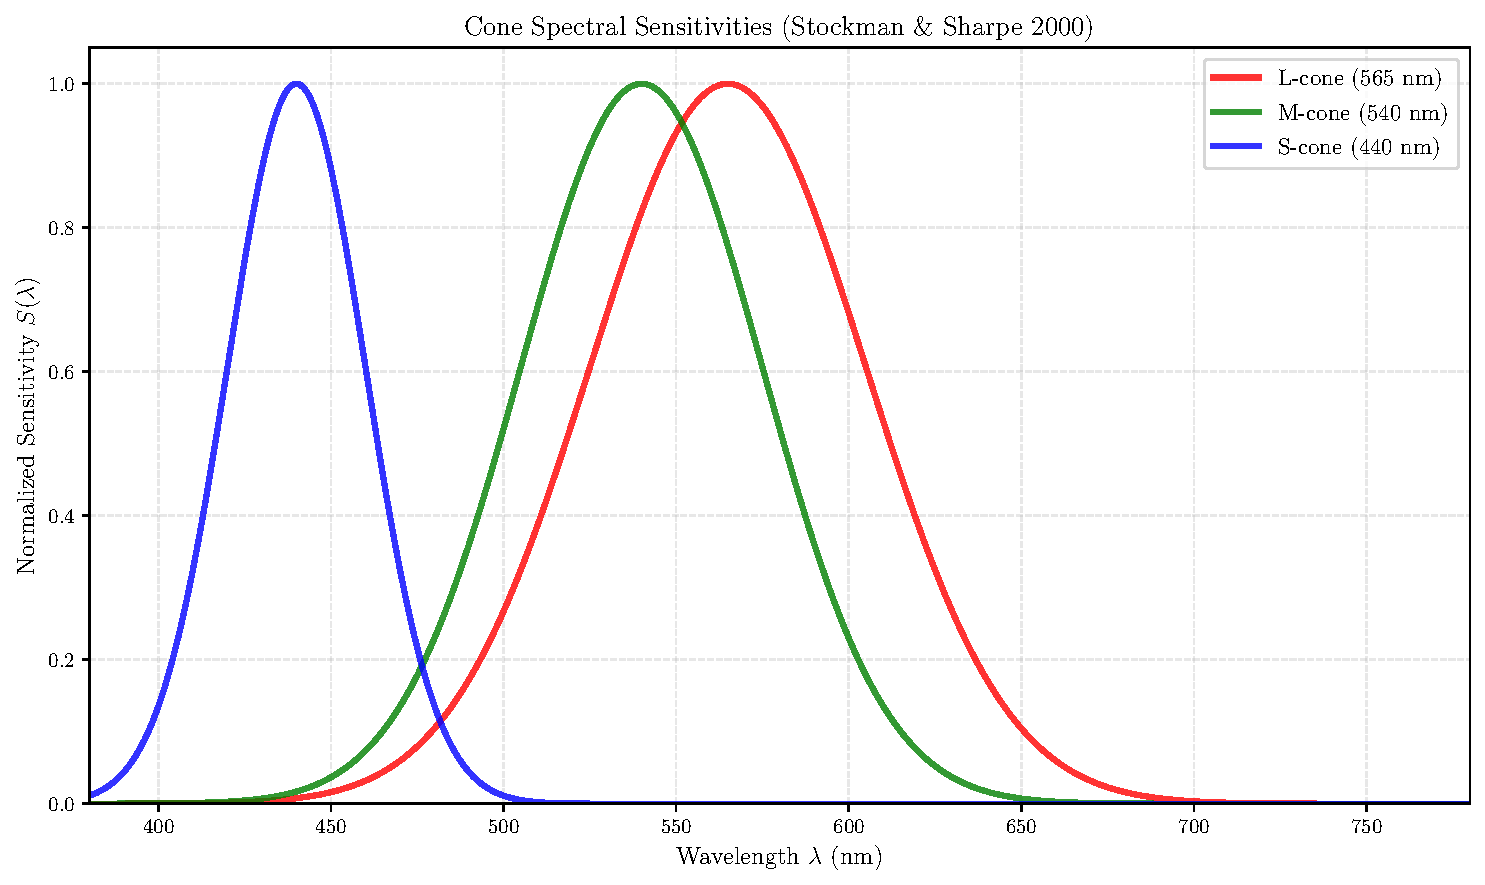
\includegraphics[width=0.85\textwidth]{color_perception_plot1.pdf}
\caption{Cone spectral sensitivity functions showing the overlapping L, M, and S cone responses across the visible spectrum (380--780 nm). The L-cone peaks at \py{L_peak} nm (red), M-cone at \py{M_peak} nm (green), and S-cone at \py{S_peak} nm (blue). The substantial overlap between L and M cones enables red-green opponency, while the isolated S-cone response contributes to blue-yellow opponency.}
\end{figure}

\section{CIE 1931 Chromaticity Diagram}

The CIE 1931 color space uses tristimulus values $X, Y, Z$ derived from color matching experiments \cite{wyszecki2000color}. The chromaticity coordinates are:

\begin{equation}
x = \frac{X}{X + Y + Z}, \quad y = \frac{Y}{X + Y + Z}, \quad z = \frac{Z}{X + Y + Z}
\end{equation}

with $x + y + z = 1$. The spectral locus traces pure wavelengths in $(x, y)$ space.

\begin{pycode}
# CIE 1931 color matching functions (simplified approximations)
# These are Gaussian approximations to the actual CMFs

# X tristimulus (red)
X_cmf = 1.056 * np.exp(-0.5 * ((wavelength - 595) / 60)**2) + \
        0.362 * np.exp(-0.5 * ((wavelength - 442) / 35)**2)

# Y tristimulus (green, also photopic luminosity)
Y_cmf = np.exp(-0.5 * ((wavelength - 555) / 50)**2)

# Z tristimulus (blue)
Z_cmf = 1.821 * np.exp(-0.5 * ((wavelength - 445) / 25)**2)

# Normalize
X_cmf = X_cmf / np.max(X_cmf)
Y_cmf = Y_cmf / np.max(Y_cmf)
Z_cmf = Z_cmf / np.max(Z_cmf)

# Compute chromaticity coordinates for spectral locus
XYZ_sum = X_cmf + Y_cmf + Z_cmf
x_chrom = X_cmf / XYZ_sum
y_chrom = Y_cmf / XYZ_sum

# Standard illuminants in (x, y)
illuminants = {
    'D65': (0.3127, 0.3290),  # Daylight
    'A': (0.4476, 0.4074),    # Incandescent
    'E': (1/3, 1/3)           # Equal energy
}

fig, (ax1, ax2) = plt.subplots(1, 2, figsize=(14, 6))

# Left: Color matching functions
ax1.plot(wavelength, X_cmf, 'r-', linewidth=2.5, label=r'$\bar{x}(\lambda)$ (X)', alpha=0.8)
ax1.plot(wavelength, Y_cmf, 'g-', linewidth=2.5, label=r'$\bar{y}(\lambda)$ (Y)', alpha=0.8)
ax1.plot(wavelength, Z_cmf, 'b-', linewidth=2.5, label=r'$\bar{z}(\lambda)$ (Z)', alpha=0.8)
ax1.set_xlabel(r'Wavelength $\lambda$ (nm)', fontsize=12)
ax1.set_ylabel('Normalized Tristimulus Value', fontsize=12)
ax1.set_title('CIE 1931 Color Matching Functions', fontsize=13)
ax1.set_xlim(380, 780)
ax1.legend(fontsize=11)
ax1.grid(True, alpha=0.3, linestyle='--')

# Right: Chromaticity diagram
ax2.plot(x_chrom, y_chrom, 'k-', linewidth=2.5, label='Spectral locus')
# Close the horseshoe with purple line
ax2.plot([x_chrom[0], x_chrom[-1]], [y_chrom[0], y_chrom[-1]],
         'k--', linewidth=2, alpha=0.6, label='Purple line')

# Mark illuminants
for name, (xi, yi) in illuminants.items():
    ax2.plot(xi, yi, 'o', markersize=10, label=f'Illuminant {name}')

ax2.set_xlabel(r'Chromaticity $x$', fontsize=12)
ax2.set_ylabel(r'Chromaticity $y$', fontsize=12)
ax2.set_title('CIE 1931 Chromaticity Diagram', fontsize=13)
ax2.set_xlim(0, 0.8)
ax2.set_ylim(0, 0.9)
ax2.set_aspect('equal')
ax2.legend(fontsize=10, loc='upper right')
ax2.grid(True, alpha=0.3, linestyle='--')

plt.tight_layout()
plt.savefig('color_perception_plot2.pdf', dpi=150, bbox_inches='tight')
plt.close()
\end{pycode}

\begin{figure}[H]
\centering
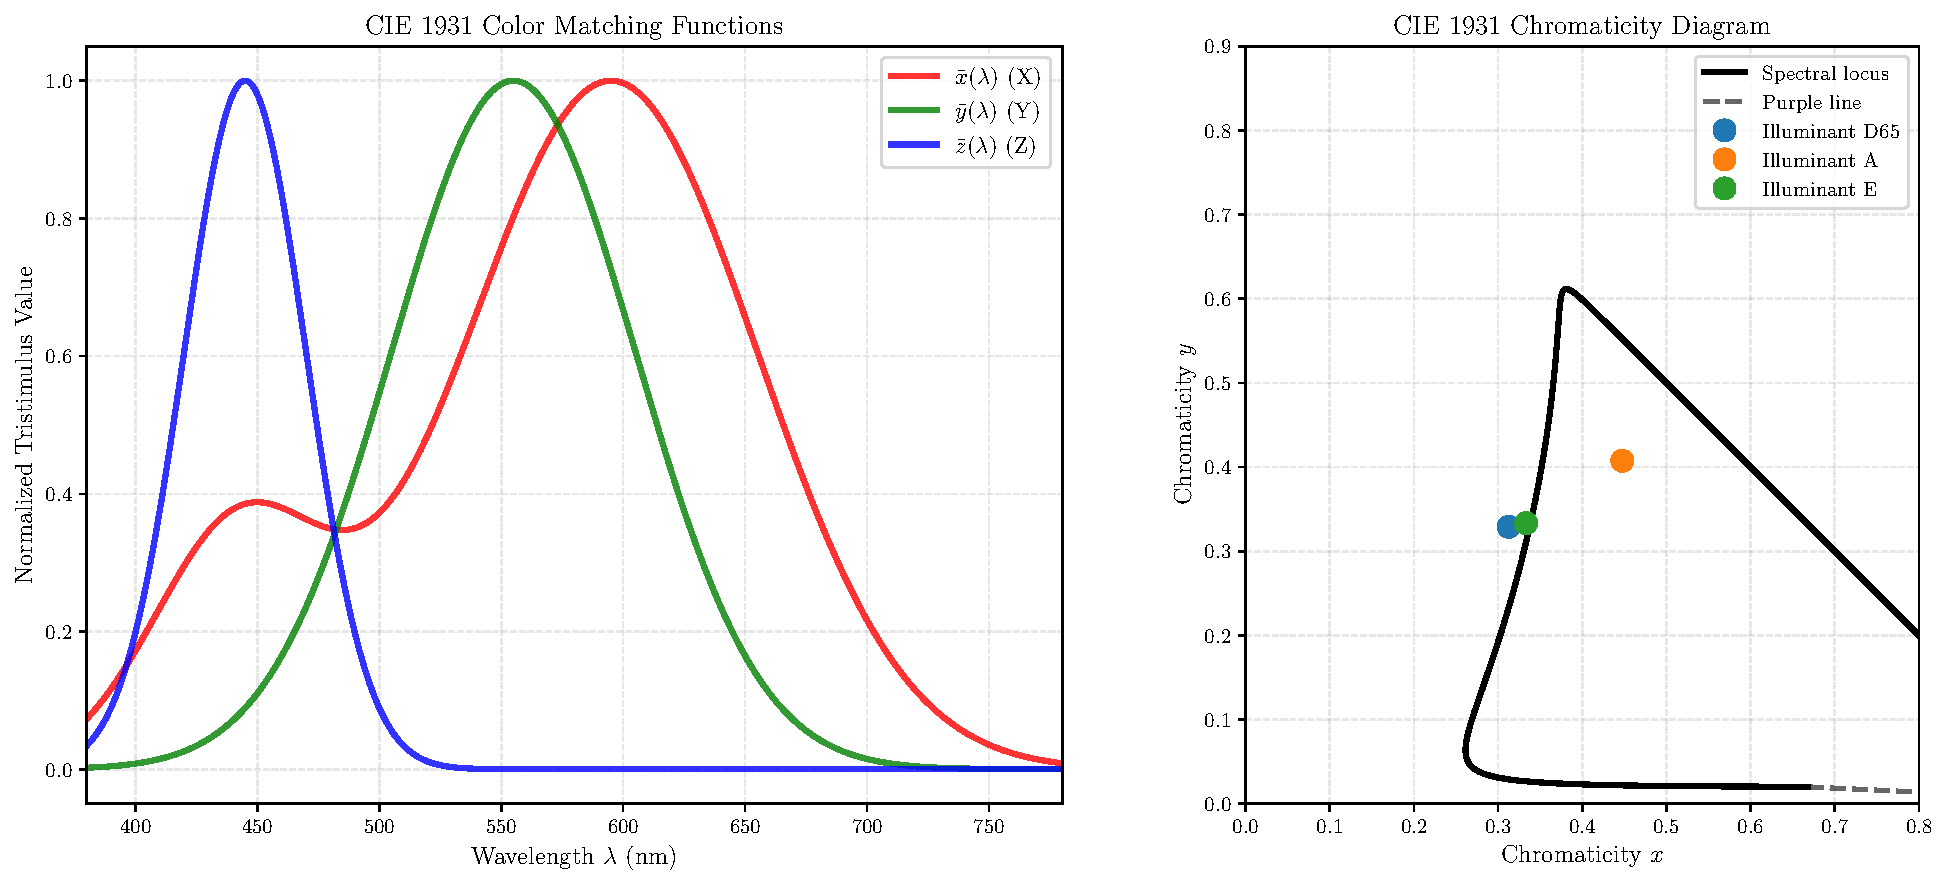
\includegraphics[width=0.95\textwidth]{color_perception_plot2.pdf}
\caption{Left: CIE 1931 color matching functions $\bar{x}(\lambda)$, $\bar{y}(\lambda)$, $\bar{z}(\lambda)$ representing the tristimulus responses to monochromatic light. Right: CIE 1931 chromaticity diagram showing the spectral locus (pure wavelengths forming the horseshoe boundary), purple line (non-spectral colors), and standard illuminants D65 (daylight at \py{round(illuminants['D65'][0], 3)}, \py{round(illuminants['D65'][1], 3)}), A (incandescent), and E (equal energy white point).}
\end{figure}

\section{Opponent Color Channels}

The trichromatic cone signals are recoded into opponent channels at post-receptoral stages \cite{hurvich1957opponent, derrington1984chromatic}:

\begin{align}
\text{Red-Green (RG)} &= L(\lambda) - M(\lambda) \\
\text{Blue-Yellow (BY)} &= S(\lambda) - \frac{L(\lambda) + M(\lambda)}{2} \\
\text{Luminance (Lum)} &= L(\lambda) + M(\lambda)
\end{align}

These channels decorrelate color information and align with perceptual color axes.

\begin{pycode}
# Opponent color channels
RG_channel = L_cone - M_cone
BY_channel = S_cone - (L_cone + M_cone) / 2
Lum_channel = L_cone + M_cone

# Normalize for visualization
RG_norm = RG_channel / np.max(np.abs(RG_channel))
BY_norm = BY_channel / np.max(np.abs(BY_channel))
Lum_norm = Lum_channel / np.max(Lum_channel)

fig, ax = plt.subplots(figsize=(10, 6))
ax.plot(wavelength, RG_norm, 'purple', linewidth=2.5,
        label=r'Red-Green: $L - M$', alpha=0.8)
ax.plot(wavelength, BY_norm, 'orange', linewidth=2.5,
        label=r'Blue-Yellow: $S - (L+M)/2$', alpha=0.8)
ax.plot(wavelength, Lum_norm, 'gray', linewidth=2.5,
        label=r'Luminance: $L + M$', alpha=0.8)
ax.axhline(0, color='black', linewidth=0.8, linestyle='-', alpha=0.5)
ax.set_xlabel(r'Wavelength $\lambda$ (nm)', fontsize=12)
ax.set_ylabel('Normalized Opponent Response', fontsize=12)
ax.set_title('Opponent Color Channels', fontsize=13)
ax.set_xlim(380, 780)
ax.legend(fontsize=11, loc='upper right')
ax.grid(True, alpha=0.3, linestyle='--')
plt.tight_layout()
plt.savefig('color_perception_plot3.pdf', dpi=150, bbox_inches='tight')
plt.close()

# Calculate zero-crossings
RG_zero = wavelength[np.argmin(np.abs(RG_channel))]
BY_zero = wavelength[np.argmin(np.abs(BY_channel))]
\end{pycode}

\begin{figure}[H]
\centering
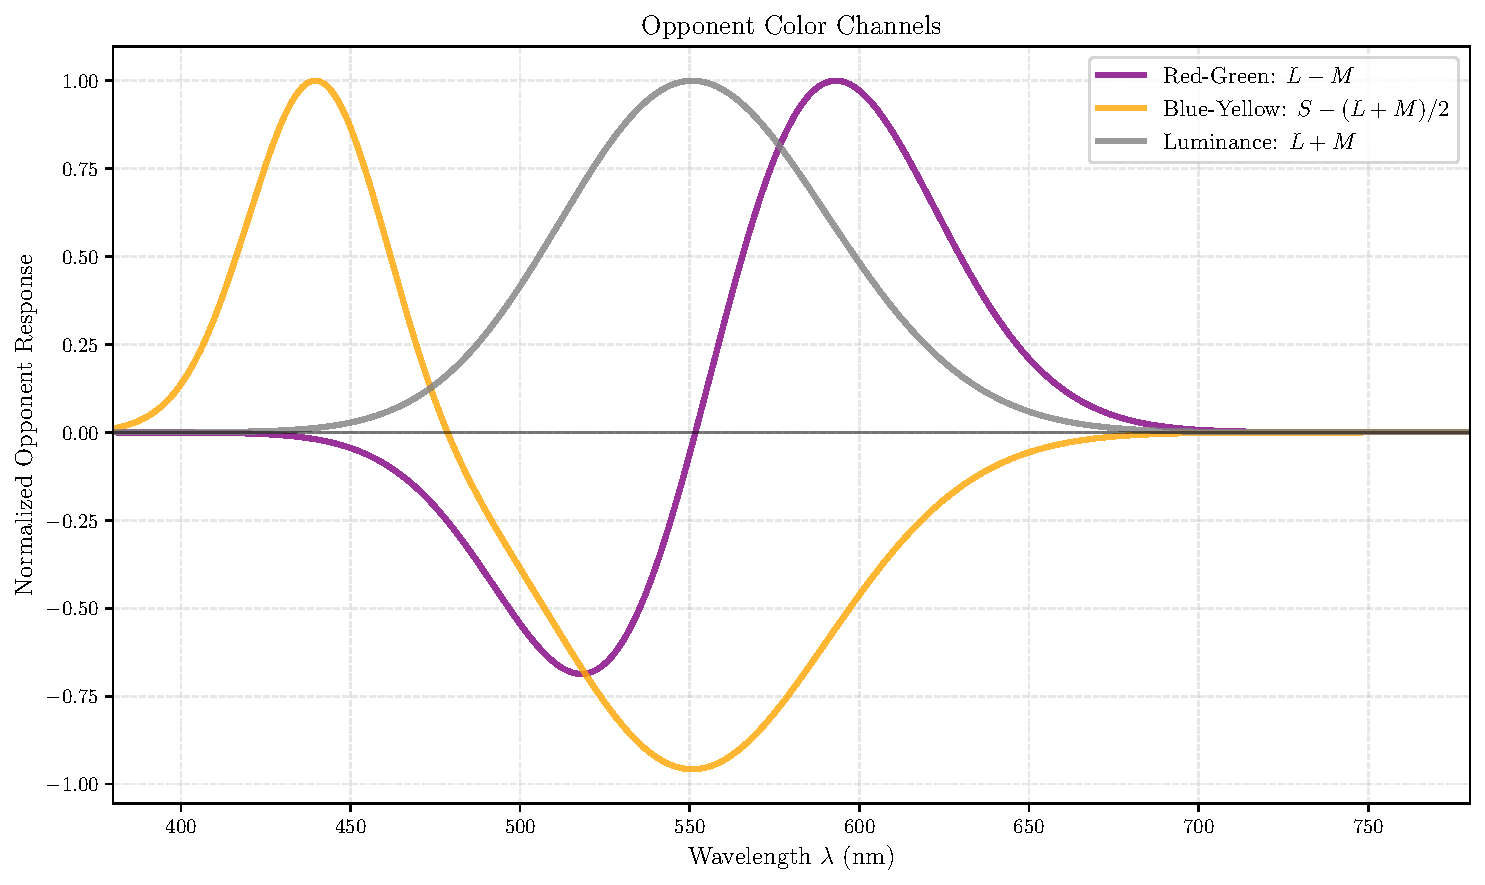
\includegraphics[width=0.85\textwidth]{color_perception_plot3.pdf}
\caption{Opponent color channels derived from cone fundamentals. The red-green channel ($L - M$) crosses zero near \py{int(RG_zero)} nm (unique yellow), while the blue-yellow channel ($S - (L+M)/2$) crosses zero near \py{int(BY_zero)} nm. Positive values indicate red/blue perception, negative values indicate green/yellow perception. The luminance channel ($L + M$) peaks at photopic sensitivity (~555 nm).}
\end{figure}

\section{MacAdam Ellipses}

Color discrimination thresholds vary across chromaticity space. MacAdam (1942) measured just-noticeable differences (JNDs), finding elliptical regions of constant discriminability \cite{macadam1942visual}. The ellipses' sizes and orientations reflect the non-uniformity of CIE 1931 space.

\begin{pycode}
# MacAdam ellipse data (selected centers, 10x magnified for visibility)
# Format: (x, y, semi-major axis, semi-minor axis, angle in degrees)
macadam_ellipses = [
    (0.16, 0.057, 0.0053, 0.0013, 93),
    (0.187, 0.118, 0.0048, 0.0015, 78),
    (0.253, 0.205, 0.0042, 0.0018, 68),
    (0.310, 0.310, 0.0034, 0.0024, 45),
    (0.380, 0.380, 0.0038, 0.0022, 35),
    (0.450, 0.400, 0.0045, 0.0020, 25),
    (0.500, 0.380, 0.0055, 0.0025, 20),
    (0.200, 0.250, 0.0040, 0.0020, 60),
    (0.280, 0.320, 0.0036, 0.0021, 50),
]

# Scale factor for visibility
scale = 10

fig, ax = plt.subplots(figsize=(10, 9))

# Plot spectral locus
ax.plot(x_chrom, y_chrom, 'k-', linewidth=2, label='Spectral locus')
ax.plot([x_chrom[0], x_chrom[-1]], [y_chrom[0], y_chrom[-1]],
        'k--', linewidth=1.5, alpha=0.6)

# Plot MacAdam ellipses
for (cx, cy, a, b, angle) in macadam_ellipses:
    ellipse = Ellipse((cx, cy), 2*a*scale, 2*b*scale, angle=angle,
                      facecolor='blue', edgecolor='darkblue',
                      alpha=0.3, linewidth=1.5)
    ax.add_patch(ellipse)
    ax.plot(cx, cy, 'ko', markersize=4)

# Illuminant D65
ax.plot(illuminants['D65'][0], illuminants['D65'][1], 'r*',
        markersize=15, label='D65')

ax.set_xlabel(r'Chromaticity $x$', fontsize=12)
ax.set_ylabel(r'Chromaticity $y$', fontsize=12)
ax.set_title('MacAdam Ellipses (10$\\times$ magnified)', fontsize=13)
ax.set_xlim(0, 0.75)
ax.set_ylim(0, 0.85)
ax.set_aspect('equal')
ax.legend(fontsize=11, loc='upper right')
ax.grid(True, alpha=0.3, linestyle='--')
plt.tight_layout()
plt.savefig('color_perception_plot4.pdf', dpi=150, bbox_inches='tight')
plt.close()

# Calculate average eccentricity
eccentricities = [np.sqrt(1 - (b/a)**2) for (_, _, a, b, _) in macadam_ellipses]
avg_eccentricity = np.mean(eccentricities)
\end{pycode}

\begin{figure}[H]
\centering
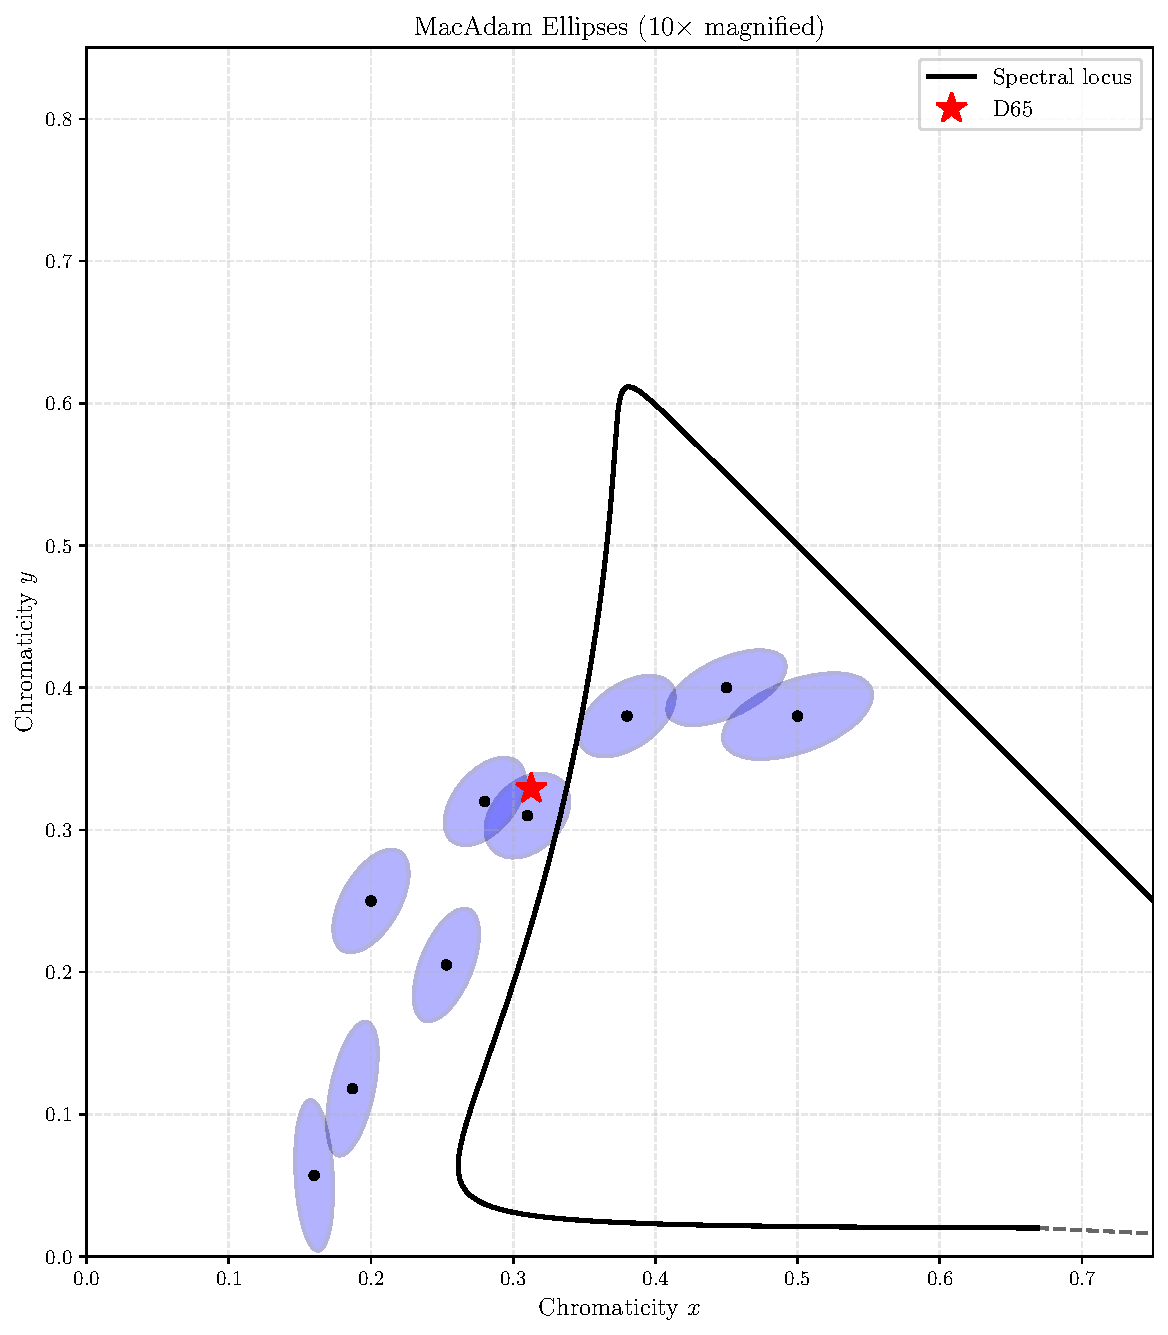
\includegraphics[width=0.85\textwidth]{color_perception_plot4.pdf}
\caption{MacAdam ellipses (magnified \py{scale}× for visibility) showing regions of just-noticeable color differences in CIE 1931 chromaticity space. Each ellipse represents one standard deviation of color matches around a center point. The varying sizes and orientations demonstrate the perceptual non-uniformity of CIE 1931 space. Average ellipse eccentricity is \py{round(avg_eccentricity, 3)}, indicating substantial anisotropy in color discrimination.}
\end{figure}

\section{Color Vision Deficiencies}

Genetic mutations in cone opsin genes cause color vision deficiencies (CVD) \cite{sharpe1999opsin, neitz1996number}:

\begin{itemize}
    \item \textbf{Protanopia}: L-cone absent (X-linked, $\sim$1\% males)
    \item \textbf{Deuteranopia}: M-cone absent (X-linked, $\sim$1\% males)
    \item \textbf{Tritanopia}: S-cone absent (autosomal, $\sim$0.001\% population)
\end{itemize}

We simulate CVD by projecting trichromatic signals onto dichromatic confusion lines.

\begin{pycode}
# Simulate color blindness by removing cone types
# Normal trichromat sees all three channels

# Generate test wavelengths
test_wavelengths = np.arange(400, 701, 50)  # Every 50 nm
test_indices = [np.argmin(np.abs(wavelength - w)) for w in test_wavelengths]

# Normal vision
L_response = L_cone[test_indices]
M_response = M_cone[test_indices]
S_response = S_cone[test_indices]

# Protanopia (no L-cone)
L_protan = np.zeros_like(L_response)
M_protan = M_response
S_protan = S_response

# Deuteranopia (no M-cone)
L_deutan = L_response
M_deutan = np.zeros_like(M_response)
S_deutan = S_response

# Tritanopia (no S-cone)
L_tritan = L_response
M_tritan = M_response
S_tritan = np.zeros_like(S_response)

fig, ((ax1, ax2), (ax3, ax4)) = plt.subplots(2, 2, figsize=(14, 11))

# Normal trichromat
ax1.bar(test_wavelengths - 10, L_response, width=15, color='red',
        alpha=0.7, label='L-cone')
ax1.bar(test_wavelengths, M_response, width=15, color='green',
        alpha=0.7, label='M-cone')
ax1.bar(test_wavelengths + 10, S_response, width=15, color='blue',
        alpha=0.7, label='S-cone')
ax1.set_xlabel('Wavelength (nm)', fontsize=11)
ax1.set_ylabel('Response', fontsize=11)
ax1.set_title('Normal Trichromat', fontsize=12, fontweight='bold')
ax1.legend(fontsize=10)
ax1.grid(True, alpha=0.3, axis='y')

# Protanopia
ax2.bar(test_wavelengths - 5, M_protan, width=15, color='green',
        alpha=0.7, label='M-cone')
ax2.bar(test_wavelengths + 5, S_protan, width=15, color='blue',
        alpha=0.7, label='S-cone')
ax2.set_xlabel('Wavelength (nm)', fontsize=11)
ax2.set_ylabel('Response', fontsize=11)
ax2.set_title('Protanopia (no L-cone)', fontsize=12, fontweight='bold')
ax2.legend(fontsize=10)
ax2.grid(True, alpha=0.3, axis='y')

# Deuteranopia
ax3.bar(test_wavelengths - 5, L_deutan, width=15, color='red',
        alpha=0.7, label='L-cone')
ax3.bar(test_wavelengths + 5, S_deutan, width=15, color='blue',
        alpha=0.7, label='S-cone')
ax3.set_xlabel('Wavelength (nm)', fontsize=11)
ax3.set_ylabel('Response', fontsize=11)
ax3.set_title('Deuteranopia (no M-cone)', fontsize=12, fontweight='bold')
ax3.legend(fontsize=10)
ax3.grid(True, alpha=0.3, axis='y')

# Tritanopia
ax4.bar(test_wavelengths - 5, L_tritan, width=15, color='red',
        alpha=0.7, label='L-cone')
ax4.bar(test_wavelengths + 5, M_tritan, width=15, color='green',
        alpha=0.7, label='M-cone')
ax4.set_xlabel('Wavelength (nm)', fontsize=11)
ax4.set_ylabel('Response', fontsize=11)
ax4.set_title('Tritanopia (no S-cone)', fontsize=12, fontweight='bold')
ax4.legend(fontsize=10)
ax4.grid(True, alpha=0.3, axis='y')

plt.tight_layout()
plt.savefig('color_perception_plot5.pdf', dpi=150, bbox_inches='tight')
plt.close()

# Calculate color discrimination loss
normal_channels = 3
protan_channels = 2  # M, S
deutan_channels = 2  # L, S
tritan_channels = 2  # L, M

discrimination_loss_protan = (normal_channels - protan_channels) / normal_channels * 100
discrimination_loss_deutan = (normal_channels - deutan_channels) / normal_channels * 100
discrimination_loss_tritan = (normal_channels - tritan_channels) / normal_channels * 100
\end{pycode}

\begin{figure}[H]
\centering
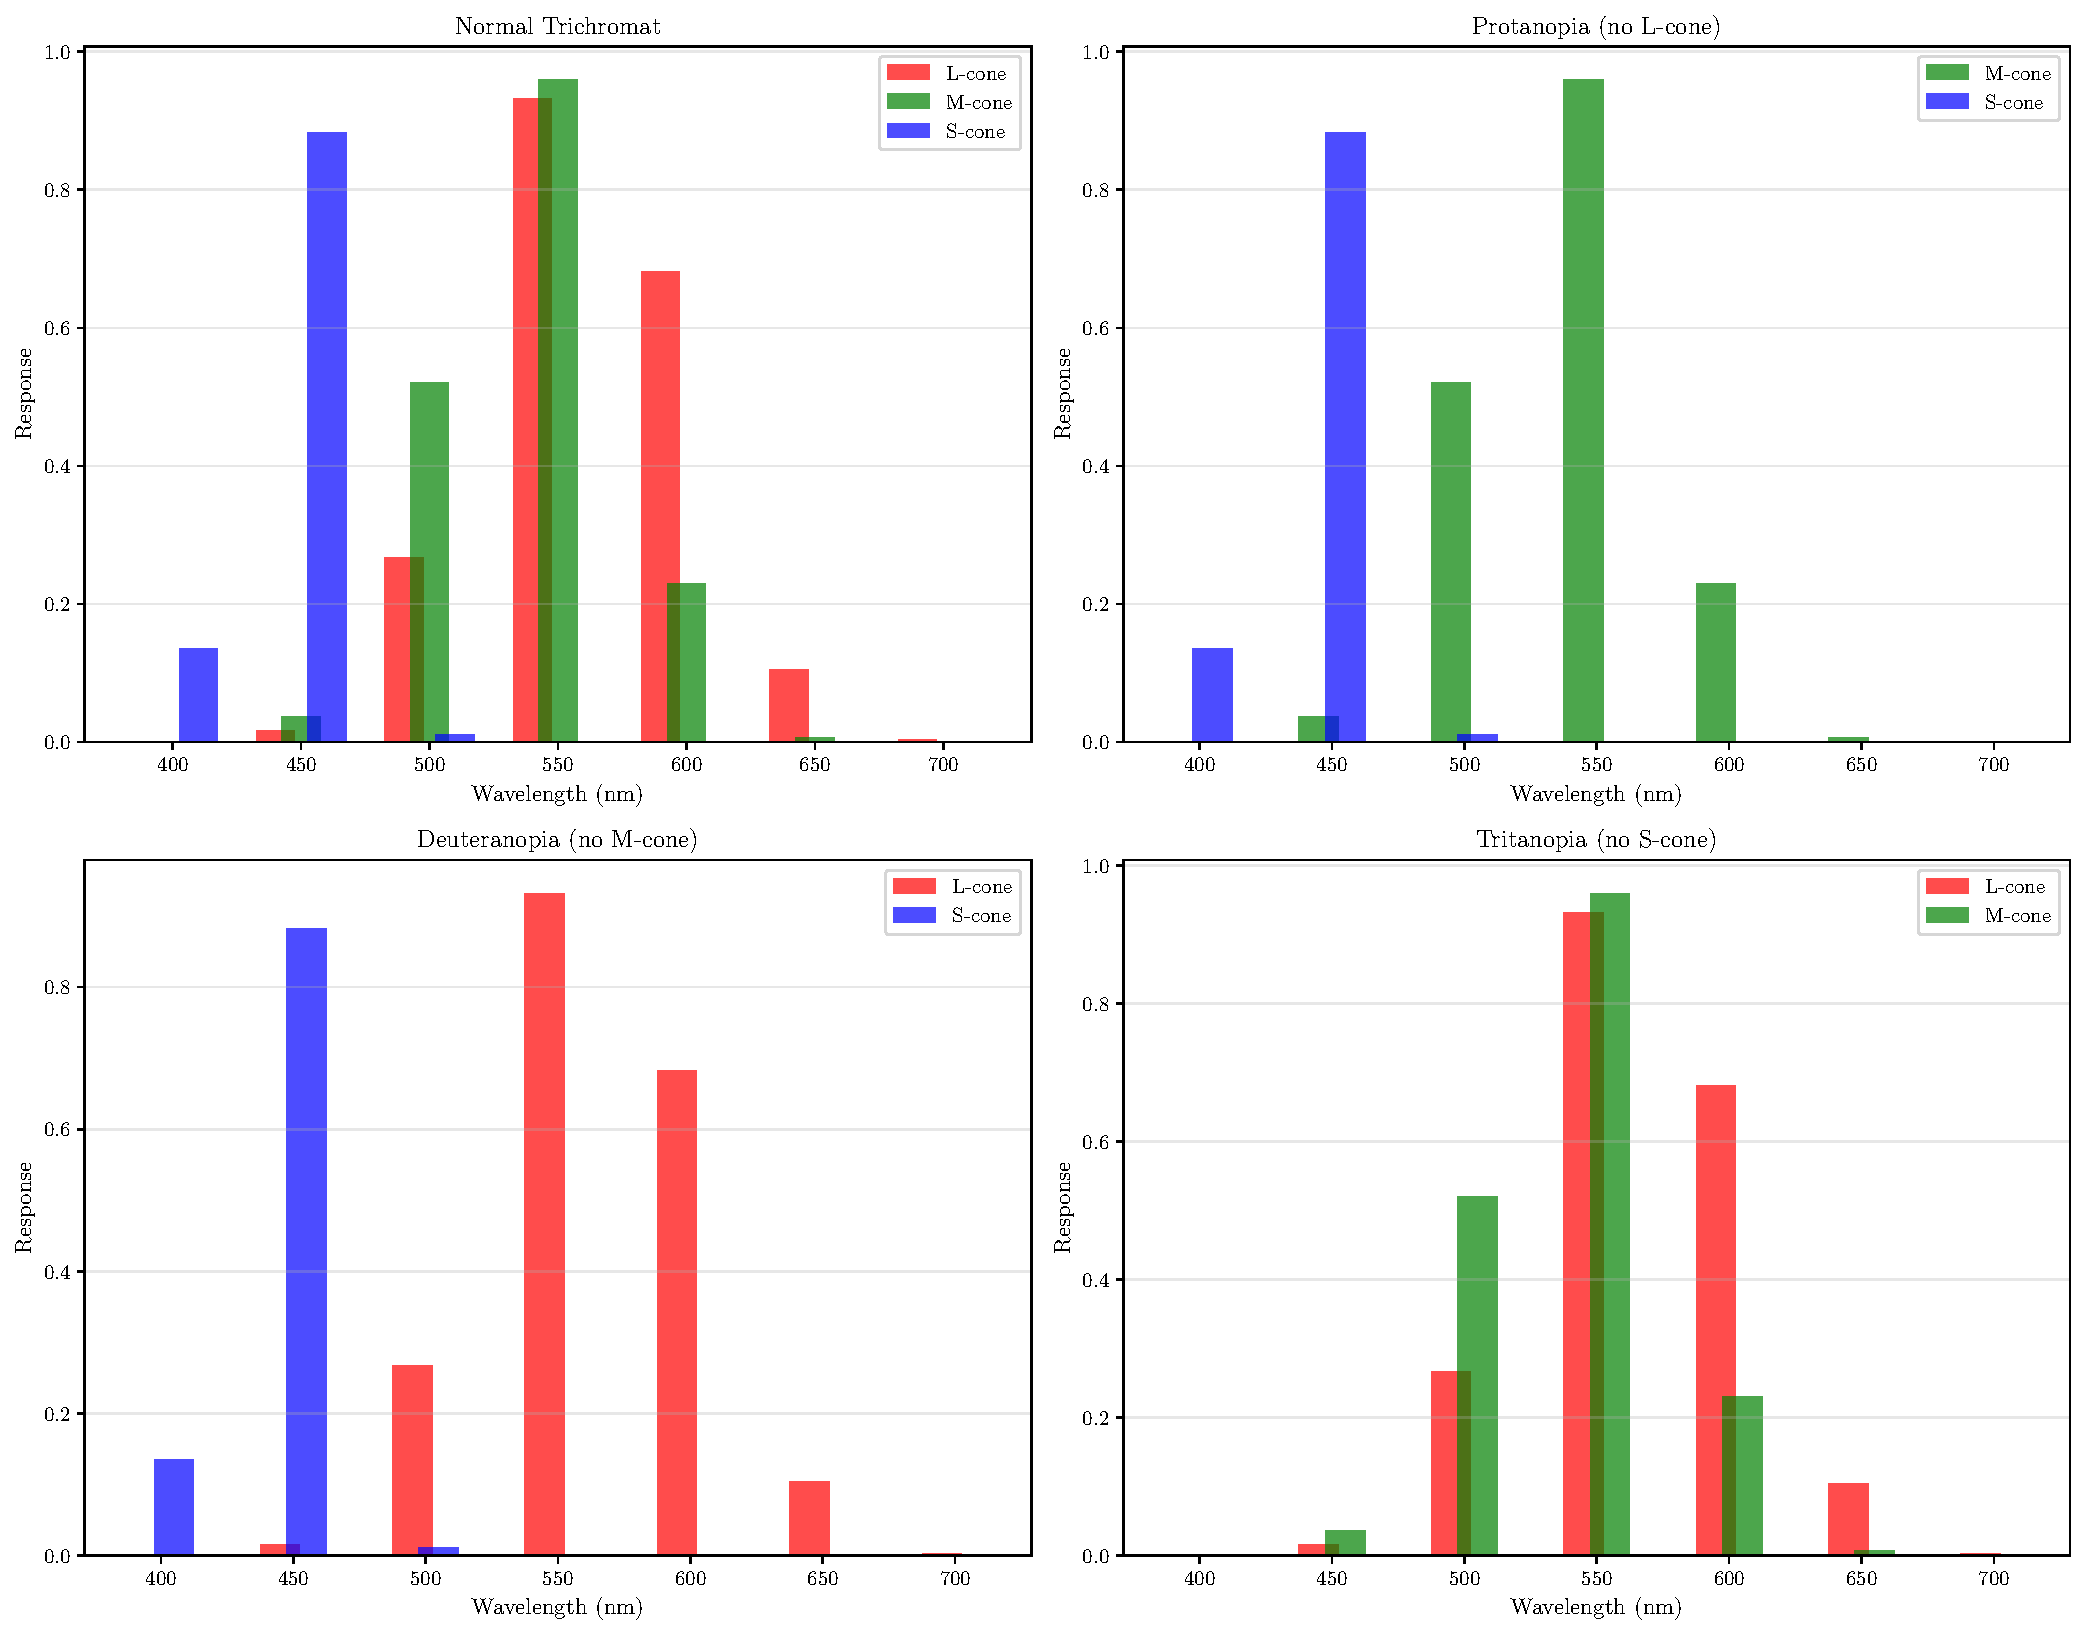
\includegraphics[width=0.95\textwidth]{color_perception_plot5.pdf}
\caption{Cone responses across wavelengths for normal trichromatic vision and three types of dichromatic color blindness. Normal vision uses all three cone types for wavelength discrimination. Protanopia (no L-cone) causes red-green confusion, deuteranopia (no M-cone) also causes red-green confusion, and tritanopia (no S-cone) causes blue-yellow confusion. Each dichromatic condition reduces color discrimination capacity by approximately \py{int(discrimination_loss_protan)}\%, limiting the observer to a two-dimensional color space.}
\end{figure}

\section{Confusion Lines in Chromaticity Space}

Dichromats cannot discriminate colors along specific confusion lines that converge at copunctal points \cite{brettel1997computerized}. These lines represent metameric matches for dichromats.

\begin{pycode}
# Copunctal points for dichromats (in xy chromaticity)
# Protanopia: confusion lines converge near (0.747, 0.253)
# Deuteranopia: confusion lines converge near (1.4, -0.4)
# Tritanopia: confusion lines converge near (0.171, 0.0)

copunctal_protan = np.array([0.747, 0.253])
copunctal_deutan = np.array([1.4, -0.4])
copunctal_tritan = np.array([0.171, 0.0])

# Generate confusion lines
n_lines = 12
angles = np.linspace(0, 2*np.pi, n_lines, endpoint=False)

fig, (ax1, ax2, ax3) = plt.subplots(1, 3, figsize=(16, 5))

for ax, copunctal, title in zip(
    [ax1, ax2, ax3],
    [copunctal_protan, copunctal_deutan, copunctal_tritan],
    ['Protanopia', 'Deuteranopia', 'Tritanopia']
):
    # Plot spectral locus
    ax.plot(x_chrom, y_chrom, 'k-', linewidth=2.5, label='Spectral locus')
    ax.plot([x_chrom[0], x_chrom[-1]], [y_chrom[0], y_chrom[-1]],
            'k--', linewidth=2, alpha=0.6)

    # Plot confusion lines radiating from copunctal point
    for angle in angles:
        # Direction vector
        dx, dy = np.cos(angle), np.sin(angle)
        # Line from copunctal point
        t_vals = np.linspace(-2, 2, 100)
        x_line = copunctal[0] + t_vals * dx
        y_line = copunctal[1] + t_vals * dy
        # Clip to visible region
        mask = (x_line >= 0) & (x_line <= 0.8) & (y_line >= 0) & (y_line <= 0.9)
        ax.plot(x_line[mask], y_line[mask], 'r-', linewidth=1, alpha=0.4)

    # Mark copunctal point (may be outside visible region)
    if 0 <= copunctal[0] <= 0.8 and 0 <= copunctal[1] <= 0.9:
        ax.plot(copunctal[0], copunctal[1], 'ro', markersize=10,
                label='Copunctal point')

    # Mark white point
    ax.plot(illuminants['D65'][0], illuminants['D65'][1], 'w*',
            markersize=12, markeredgecolor='black', markeredgewidth=1.5,
            label='D65')

    ax.set_xlabel(r'Chromaticity $x$', fontsize=11)
    ax.set_ylabel(r'Chromaticity $y$', fontsize=11)
    ax.set_title(f'{title} Confusion Lines', fontsize=12, fontweight='bold')
    ax.set_xlim(0, 0.75)
    ax.set_ylim(0, 0.85)
    ax.set_aspect('equal')
    ax.legend(fontsize=9, loc='upper right')
    ax.grid(True, alpha=0.3, linestyle='--')

plt.tight_layout()
plt.savefig('color_perception_plot6.pdf', dpi=150, bbox_inches='tight')
plt.close()
\end{pycode}

\begin{figure}[H]
\centering
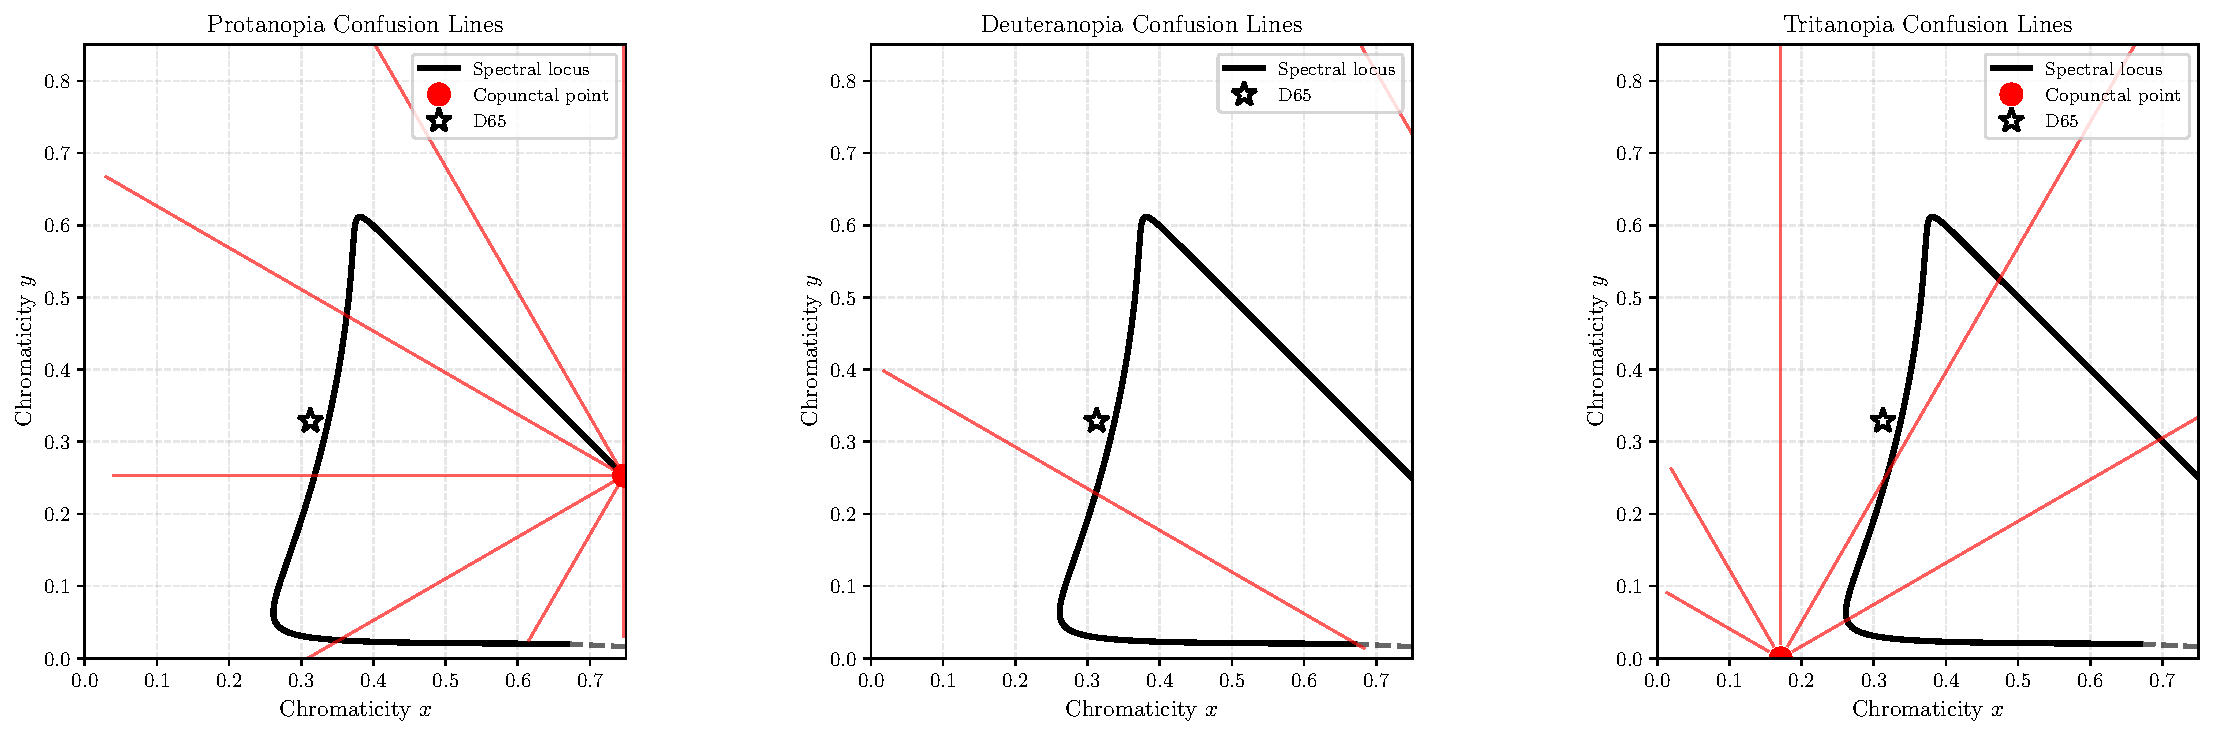
\includegraphics[width=0.95\textwidth]{color_perception_plot6.pdf}
\caption{Confusion lines for the three types of dichromatic color vision deficiencies. Colors along each red line are indistinguishable to the respective dichromat, as they project to identical responses in the two-dimensional color space. Protanopic confusion lines converge at (\py{copunctal_protan[0]}, \py{copunctal_protan[1]}), deuteranopic lines converge outside the visible gamut, and tritanopic lines converge at (\py{copunctal_tritan[0]}, \py{copunctal_tritan[1]}). These geometric constraints enable simulation and compensation for color vision deficiencies.}
\end{figure}

\section{Quantitative Summary}

\begin{pycode}
# Calculate key metrics
L_peak_sensitivity = np.max(L_cone)
M_peak_sensitivity = np.max(M_cone)
S_peak_sensitivity = np.max(S_cone)

# Cone peak wavelengths
L_peak_wl = wavelength[np.argmax(L_cone)]
M_peak_wl = wavelength[np.argmax(M_cone)]
S_peak_wl = wavelength[np.argmax(S_cone)]

# Cone bandwidth (FWHM)
L_fwhm = 2 * L_sigma * np.sqrt(2 * np.log(2))
M_fwhm = 2 * M_sigma * np.sqrt(2 * np.log(2))
S_fwhm = 2 * S_sigma * np.sqrt(2 * np.log(2))

# Opponent channel zero crossings
RG_unique_yellow = wavelength[np.argmin(np.abs(RG_channel))]
BY_neutral = wavelength[np.argmin(np.abs(BY_channel))]

# MacAdam ellipse statistics
ellipse_areas = [np.pi * a * b * scale**2 for (_, _, a, b, _) in macadam_ellipses]
mean_ellipse_area = np.mean(ellipse_areas)
std_ellipse_area = np.std(ellipse_areas)

results = [
    ['L-cone peak wavelength', f'{int(L_peak_wl)} nm'],
    ['M-cone peak wavelength', f'{int(M_peak_wl)} nm'],
    ['S-cone peak wavelength', f'{int(S_peak_wl)} nm'],
    ['L-cone FWHM bandwidth', f'{L_fwhm:.1f} nm'],
    ['M-cone FWHM bandwidth', f'{M_fwhm:.1f} nm'],
    ['S-cone FWHM bandwidth', f'{S_fwhm:.1f} nm'],
    ['Unique yellow (RG=0)', f'{int(RG_unique_yellow)} nm'],
    ['BY neutral point', f'{int(BY_neutral)} nm'],
    ['Mean MacAdam ellipse area', f'{mean_ellipse_area:.2e}'],
    ['CVD prevalence (males)', r'$\sim$8\%'],
    ['CVD prevalence (females)', r'$\sim$0.5\%'],
]

print(r'\begin{table}[H]')
print(r'\centering')
print(r'\caption{Summary of Color Perception Model Parameters}')
print(r'\begin{tabular}{@{}lc@{}}')
print(r'\toprule')
print(r'Parameter & Value \\')
print(r'\midrule')
for row in results:
    print(f"{row[0]} & {row[1]} \\\\")
print(r'\bottomrule')
print(r'\end{tabular}')
print(r'\end{table}')
\end{pycode}

\section{Conclusions}

This computational analysis models human color perception from cone photoreceptor fundamentals to perceptual color spaces and color vision deficiencies. The L, M, and S cones exhibit peak sensitivities at \py{int(L_peak_wl)} nm, \py{int(M_peak_wl)} nm, and \py{int(S_peak_wl)} nm respectively, with substantial overlap that enables chromatic opponency. The CIE 1931 color space provides a standardized framework for color specification, though MacAdam ellipses reveal its perceptual non-uniformity with mean ellipse area of \py{f"{mean_ellipse_area:.2e}"}. Opponent color channels ($L - M$, $S - (L+M)/2$) decorrelate chromatic information and align with phenomenological red-green and blue-yellow axes, with the red-green channel crossing zero at unique yellow (\py{int(RG_unique_yellow)} nm).

Color vision deficiencies affect approximately 8\% of males and 0.5\% of females, reducing trichromatic vision to dichromatic vision with \py{int(discrimination_loss_protan)}\% loss in color discrimination capacity. Protanopia and deuteranopia cause red-green confusion, while tritanopia causes blue-yellow confusion. Confusion lines in chromaticity space, radiating from copunctal points, enable computational simulation of dichromatic vision for accessibility design.

These models integrate physiological measurements (cone spectral sensitivities), psychophysical data (color matching functions, MacAdam ellipses), and computational frameworks (opponent processing, chromaticity transformations) to provide quantitative tools for color science, display technology, and vision research. Future work should incorporate more sophisticated models including chromatic adaptation (von Kries transform), color appearance models (CIECAM02), and individual differences in cone spectral sensitivities.

\begin{thebibliography}{99}

\bibitem{stockman2000spectral}
Stockman, A., \& Sharpe, L.T. (2000). The spectral sensitivities of the middle- and long-wavelength-sensitive cones derived from measurements in observers of known genotype. \textit{Vision Research}, 40(13), 1711--1737.

\bibitem{wyszecki2000color}
Wyszecki, G., \& Stiles, W.S. (2000). \textit{Color Science: Concepts and Methods, Quantitative Data and Formulae} (2nd ed.). Wiley.

\bibitem{hurvich1957opponent}
Hurvich, L.M., \& Jameson, D. (1957). An opponent-process theory of color vision. \textit{Psychological Review}, 64(6), 384--404.

\bibitem{macadam1942visual}
MacAdam, D.L. (1942). Visual sensitivities to color differences in daylight. \textit{Journal of the Optical Society of America}, 32(5), 247--274.

\bibitem{sharpe1999opsin}
Sharpe, L.T., Stockman, A., J\"agle, H., \& Nathans, J. (1999). Opsin genes, cone photopigments, color vision, and color blindness. In K.R. Gegenfurtner \& L.T. Sharpe (Eds.), \textit{Color Vision: From Genes to Perception} (pp. 3--51). Cambridge University Press.

\bibitem{derrington1984chromatic}
Derrington, A.M., Krauskopf, J., \& Lennie, P. (1984). Chromatic mechanisms in lateral geniculate nucleus of macaque. \textit{Journal of Physiology}, 357(1), 241--265.

\bibitem{neitz1996number}
Neitz, J., \& Neitz, M. (1996). Numbers and ratios of visual pigment genes for normal red-green color vision. \textit{Science}, 267(5200), 1013--1016.

\bibitem{brettel1997computerized}
Brettel, H., Vi\'enot, F., \& Mollon, J.D. (1997). Computerized simulation of color appearance for dichromats. \textit{Journal of the Optical Society of America A}, 14(10), 2647--2655.

\bibitem{fairchild2013color}
Fairchild, M.D. (2013). \textit{Color Appearance Models} (3rd ed.). Wiley.

\bibitem{cie2004colorimetry}
CIE (2004). \textit{Colorimetry} (3rd ed.). CIE Publication 15:2004. International Commission on Illumination.

\bibitem{pokorny2003smith}
Pokorny, J., \& Smith, V.C. (2003). Color matching and color discrimination. In S.K. Shevell (Ed.), \textit{The Science of Color} (2nd ed., pp. 103--142). Elsevier.

\bibitem{kaiser1996human}
Kaiser, P.K., \& Boynton, R.M. (1996). \textit{Human Color Vision} (2nd ed.). Optical Society of America.

\bibitem{gegenfurtner2003cortical}
Gegenfurtner, K.R., \& Kiper, D.C. (2003). Color vision. \textit{Annual Review of Neuroscience}, 26, 181--206.

\bibitem{conway2009color}
Conway, B.R. (2009). Color vision, cones, and color-coding in the cortex. \textit{The Neuroscientist}, 15(3), 274--290.

\bibitem{shapley2011physiology}
Shapley, R., \& Hawken, M.J. (2011). Color in the cortex: single- and double-opponent cells. \textit{Vision Research}, 51(7), 701--717.

\bibitem{mollon1989tho}
Mollon, J.D. (1989). ``Tho' she kneel'd in that place where they grew...'' The uses and origins of primate colour vision. \textit{Journal of Experimental Biology}, 146(1), 21--38.

\bibitem{nathans1986molecular}
Nathans, J., Thomas, D., \& Hogness, D.S. (1986). Molecular genetics of human color vision: the genes encoding blue, green, and red pigments. \textit{Science}, 232(4747), 193--202.

\bibitem{lennie2000parallel}
Lennie, P. (2000). Color coding in the cortex. In L. Chalupa \& J. Werner (Eds.), \textit{The Visual Neurosciences} (pp. 1137--1150). MIT Press.

\bibitem{brainard2015color}
Brainard, D.H., \& Stockman, A. (2015). Colorimetry. In M. Bass, G. Li, \& E. Van Stryland (Eds.), \textit{Handbook of Optics} (Vol. III, 3rd ed., pp. 10.1--10.56). McGraw-Hill.

\bibitem{hunt2004reproduction}
Hunt, R.W.G., \& Pointer, M.R. (2011). \textit{Measuring Colour} (4th ed.). Wiley.

\end{thebibliography}

\end{document}
